\documentclass{article}
\usepackage{tabularx, booktabs, graphicx}

\usepackage{geometry}
 \geometry{
 left=10mm,
 top=10mm,
 }
 
\begin{document}
\pagenumbering{gobble}
\oddsidemargin-1cm
\textwidth19cm
\begin{table}
\setlength\tabcolsep{6pt} % default value: 6pt
\centering
\begin{tabularx}{\textwidth}{m{5.6cm} m{3.4cm} m{5.6cm} m{3.4cm}}
 
\hline
\toprule
\multicolumn{4}{c}{Community-level predictions} \\
\midrule
\hline
\toprule
Prediction & Pattern & Prediction & Pattern\\ [0.5ex]
\midrule

1. Total abundance (\textit{N}) should be lowest at low $\tau$ due to washout and at high $\tau$ due to low resource resupply.
&
\begin{minipage}{.3\textwidth}
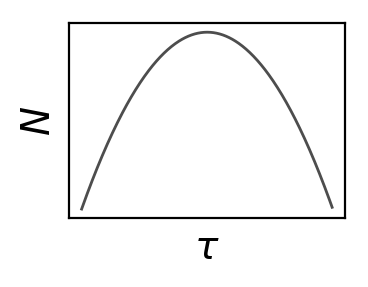
\includegraphics[width=30mm, height=25mm]{predictions/N}
\end{minipage}
&
2. Productivity (\textit{P}) should be lowest at low $\tau$ due to washout and at high $\tau$ due to low resource resupply.
&
\begin{minipage}{.3\textwidth}
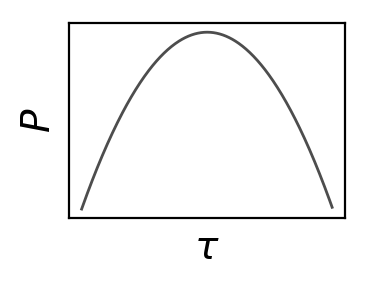
\includegraphics[width=30mm, height=25mm]{predictions/P}
\end{minipage} \\
    
\addlinespace
3. Species richness (\textit{S}) should be lowest at low $\tau$ due to selection to resist washout and at high $\tau$ due to selection on persistence.
&
\begin{minipage}{.3\textwidth}
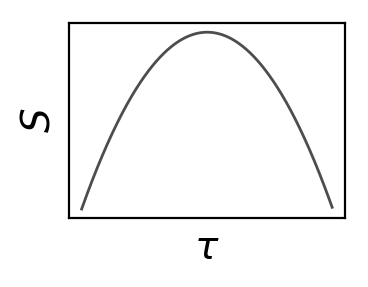
\includegraphics[width=30mm, height=25mm]{predictions/S}
\end{minipage}
&
4. Species evenness (\textit{E}) should be lowest at intermediate $\tau$, reflecting competition and the constraining influence of \textit{N} and \textit{S}.
&
\begin{minipage}{.3\textwidth}
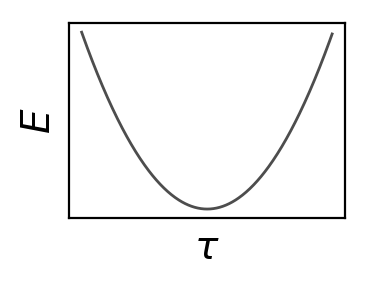
\includegraphics[width=30mm, height=25mm]{predictions/E}
\end{minipage} \\
 
\addlinespace
5. Species turnover (\textit{W}) should decrease with greater $\tau$, reflecting less immigration and greater persistence. \textit{W} may then increase, due to loss of species at low \textit{S}.
&
\begin{minipage}{.3\textwidth}
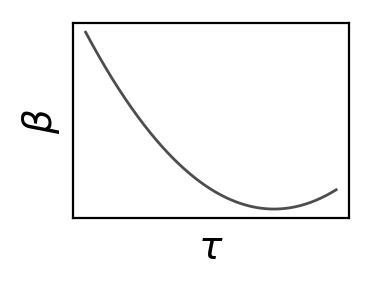
\includegraphics[width=30mm, height=25mm]{predictions/Beta}
\end{minipage}
&
6. The percent of individuals in a dormant state should increase with greater $\tau$ due to insufficient resource resupply and decreased threat of washout.
&
\begin{minipage}{.3\textwidth}
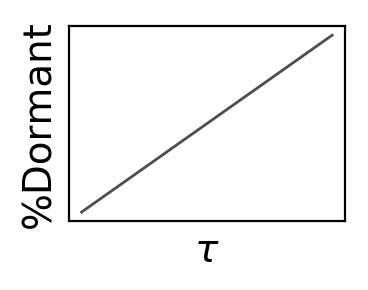
\includegraphics[width=30mm, height=25mm]{predictions/D}
\end{minipage} \\
 
\hline
\toprule
\multicolumn{4}{c}{Trait-level predictions} \\ 
\midrule
\hline
\toprule
Prediction & Pattern & Prediction & Pattern\\ [0.5ex]
\midrule

\addlinespace
7. Intrinsic rates of growth should decrease with greater $\tau$, reflecting of growing quickly in rapidly moving systems and of growing less quickly in resource deplete conditions.
&
\begin{minipage}{.3\textwidth}
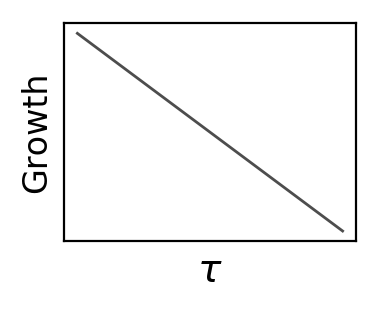
\includegraphics[width=30mm, height=25mm]{predictions/Growth}
\end{minipage}
&
8. Active basal metabolic rate ($B$) should decrease with greater $\tau$, reflecting pressures to accomplish similar rates of energeticaly costly processes at lower energetic costs.
&
\begin{minipage}{.3\textwidth}
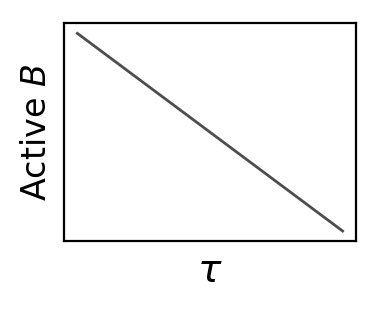
\includegraphics[width=30mm, height=25mm]{predictions/BMR}
\end{minipage} \\
 
\addlinespace
9. Rates of active dispersal should decrease with greater $\tau$, reflecting advantages of strong dispersal in rapidly moving systems and the costs of active dispersal in resource deplete systems.
&
\begin{minipage}{.3\textwidth}
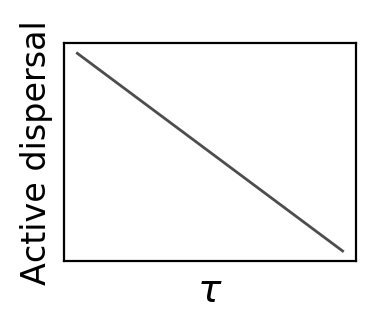
\includegraphics[width=30mm, height=25mm]{predictions/Dispersal}
\end{minipage}
&
10. Resource specialization should should be low at short and long $\tau$. Specialization should increase as resource partitioning emerges among greaters numbers of competing species.
&
\begin{minipage}{.3\textwidth}
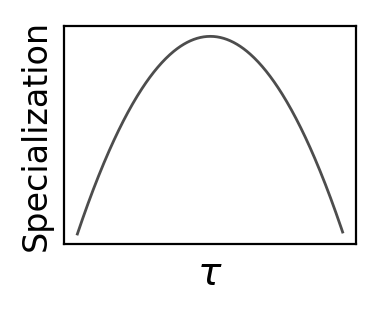
\includegraphics[width=30mm, height=25mm]{predictions/Spec}
\end{minipage} \\
 
\addlinespace
11. Rates of resuscitation from dormancy should decrease with greater $\tau$, reflecting the disadvantage of being dormant at short $\tau$ and the costs of active metabolism at long $\tau$.
&
\begin{minipage}{.3\textwidth}
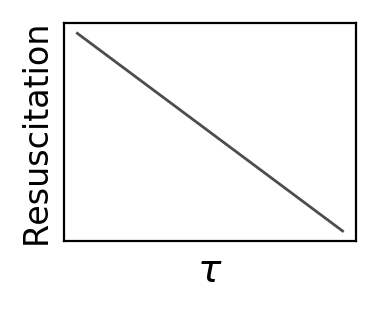
\includegraphics[width=30mm, height=25mm]{predictions/Resus}
\end{minipage}
&
12. Increasing $\tau$ should select for a greater reduction of basal metabolic rate ($B$) when individuals go dormant.
&
\begin{minipage}{.3\textwidth}
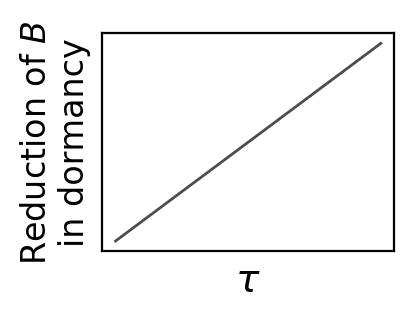
\includegraphics[width=30mm, height=25mm]{predictions/ReducB}
\end{minipage} \\
 
\hline
\toprule
\multicolumn{4}{c}{Equivalence predictions} \\ 
\midrule
\hline
\toprule
Prediction & Pattern & Prediction & Pattern\\ [0.5ex]
\midrule

\addlinespace
13. The difference between the rates of energetically costly traits $T$ and $1/\tau$ represents the match between resource supply and energetic costs. \textit{N} should be greatest when $T$ = $1/\tau$.
&
\begin{minipage}{.3\textwidth}
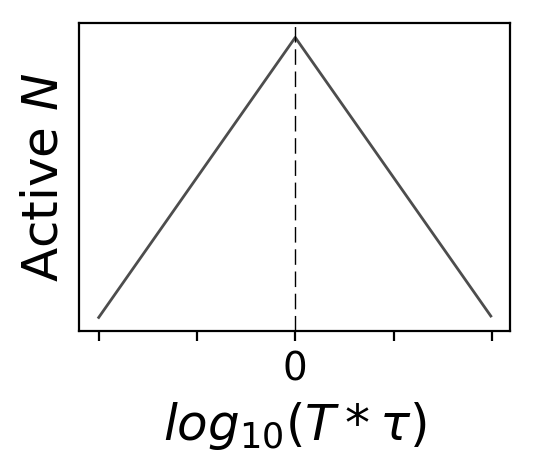
\includegraphics[width=30mm, height=25mm]{predictions/N-equiv}
\end{minipage}
&
14. The difference between the rates of energetically costly traits $T$ and $1/\tau$ represents the match between resource supply and energetic costs. \textit{P} should be greatest when $T$ = $1/\tau$.
&
\begin{minipage}{.3\textwidth}
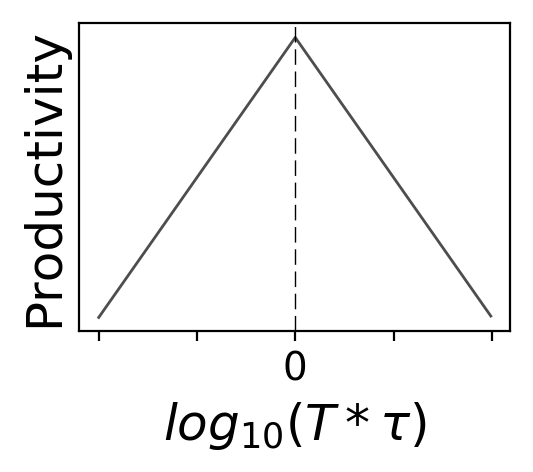
\includegraphics[width=30mm, height=25mm]{predictions/P-equiv}
\end{minipage} \\
\hline

\end{tabularx}
\end{table}
\end{document}